\documentclass{article}


\usepackage{arxiv}

\usepackage[utf8]{inputenc} % allow utf-8 input
\usepackage[T1]{fontenc}    % use 8-bit T1 fonts
\usepackage{hyperref}       % hyperlinks
\usepackage{url}            % simple URL typesetting
\usepackage{booktabs}       % professional-quality tables
\usepackage{amsfonts}       % blackboard math symbols
\usepackage{nicefrac}       % compact symbols for 1/2, etc.
\usepackage{microtype}      % microtypography
\usepackage{lipsum}
\usepackage{enumitem}
\usepackage[polish]{babel}  % English language hyphenation
\usepackage{float}          % for H in \begin{figure}[H]. Force including file in place.
\usepackage{caption}
\usepackage{subcaption}
\usepackage{placeins}
\usepackage{graphicx}
\usepackage{lmodern}
\graphicspath{./images/}

%\fancyhf{} % sets both header and footer to nothing
\renewcommand{\headrulewidth}{0pt}
% your new footer definitions here

\newcommand{\todo}[1]{\textcolor{red}{TODO: #1}}

% kolory odnośników
\usepackage[dvipsnames]{xcolor}
\hypersetup{
    colorlinks=true,
    linkcolor=black,
    filecolor=black,
    citecolor=black,
    urlcolor=cyan,
    pdftitle={Sharelatex Example},
    pdfpagemode=FullScreen,
}
\urlstyle{same}


\title{Kwantyzacja wektorowa}

\author{
  Karol Działowski \\
  \textbf{Wojciech Olejnik} \\
  \textbf{Paweł Kalicki} \\
  Zachodniopomorski Uniwersytet Technologiczny
}

\begin{document}
\maketitle
\begin{abstract}
\lipsum[1-2]
\end{abstract}

\newpage

\tableofcontents

\newpage

% keywords can be removed
%\keywords{First keyword \and Second keyword \and More}


\section{Wstęp}

Kwantyzacja polega na przyporządkowaniu wartościom sygnału ciągłego wartości dyskretnych należących do skończonego zbioru.
Przedział wartości sygnału dzielony jest na zbiór przedziałów.
Zazwyczaj przedziały mają taką samą wielkość (kwantyzacja liniowa).
Stosuje się też kwantyzację nieliniową, gdzie przedziały nie są równomiernie podzielone. 

Z każdym przedziałem powiązany jest określony poziom kwantyzacji. 
Gdy wartość sygnału wejściowego należy do danego przedziału przyporządkowuje mu się odpowiednią wartość kwantyzacji.

Podczas procesu kwantyzacji powstają błędy kwantyzacji wynikające z różnicy rzeczywistej wartości od wartości kwantyzacji. 
Błędy te objawiają się w postaci tak zwanego szumu kwantyzacji. 
Im większe przedziały kwantyzacji tym mniejsza jej dokładność i tym większy jest szum kwantyzacji. 
W przetwarzaniu analogowo-cyfrowym dokładność liniowej kwantyzacji jest określona przez liczbę bitów wykorzystywanych do zapisu skwantyzowanej wartości. 
Zwiększenie liczby bitów prowadzi do zwiększenia liczby przedziałów, co w rezultacie prowadzi do dokładniejszego odwzorowania \mbox{sygnału \cite{drozdek2007wprowadzenie}.}

\section{Opis projektu}

Celem projektu było stworzenie aplikacji umożliwiającej przeprowadzanie kwantyzacji wektorowej oraz przeprowadzenie badań
zaimplementowanych metod.

\subsection{Kwantyzacja wektorowa}
Kwantyzacja wektorowa (ang. \emph{vector quantization}) polega na podziale wielowymiarowych przestrzeni na obszary i
przyporządkowanie każdemu obszarowi odpowiedniego poziomu kwantyzacji.
Obszary reprezentowanego są w formie wektorów.
Przykładem zastosowania kwantyzacji wektorowej jest kompresja obrazów.

W celu kwantyzacji obraz dzielony jest na obszary o zadanym rozmiarze, np. $4 \times 4$ pikseli, co tworzy wektory o długości $16$.
Budowana jest książka kodowa reprezentująca poziomy kwantyzacji na podstawie wyznacznych wektorów.
Dla każdego obszaru detekcyjnego przyporządkowuje się indeks wyznaczonego najbliższego poziomu kwantyzacji.

Jakość kwantyzacji zależy od długości wektorów i doboru książki kodowej (procesu jego budowy i długości).

\begin{figure}[H]
    \centering
    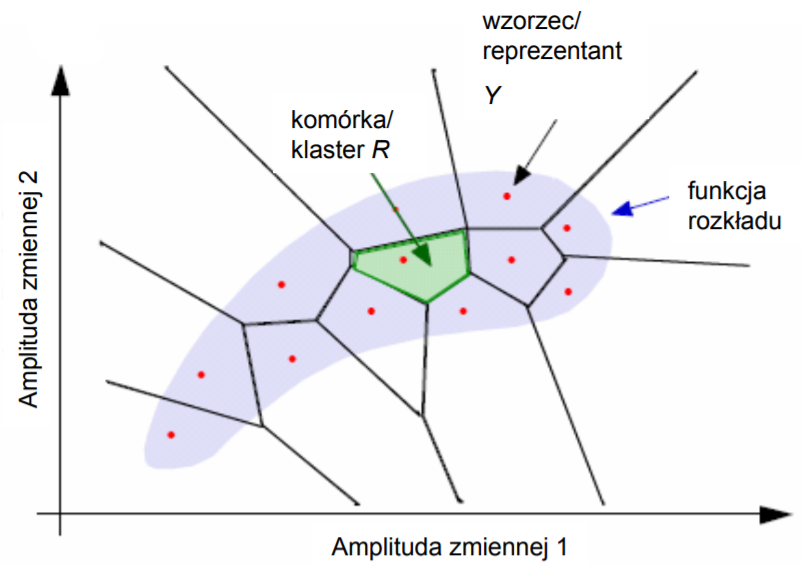
\includegraphics[width=0.6\textwidth]{images/kwantyzacja_wektorowa.png}
    \caption{Przykład podziału dwuwymiarowej przestrzeni danych na klastry grupujące według słownika. Źródło \cite{mwilczewski}.}
    \label{fig:kwantyzacja_wektorowa}
\end{figure}

\subsection{Ogólny przebieg etapów pracy kwantyzatora wektorowego}

\begin{enumerate}
  \item Formowanie danych wejściowych do postaci $N$ wektorów $n$ -- wymiarowych (etap wstępny). 
  \item Faza klasteryzacji: podział wszystkich wektorów wejściowych i konstrukcja książki 
    kodowej (słownika) zawierającej $K$ najbardziej reprezentatywnych wektorów całego zbioru danych, 
    tzw. wektorów kodowych. Konstrukcja książki kodowej może być wykonana w fazie wstępnej na podstawie zbioru 
    treningowego lub dynamicznie we właściwej fazie kwantyzacji. Faza klasteryzacji jest kluczowym etapem kwantyzacji wektorowej.
  \item Faza indeksowania: przyporządkowanie każdemu wektorowi wejściowemu jednego wektora ze słownika i reprezentowanie wektora wejściowego indeksem słownika. 
\end{enumerate}

\begin{figure}[H]
    \centering
    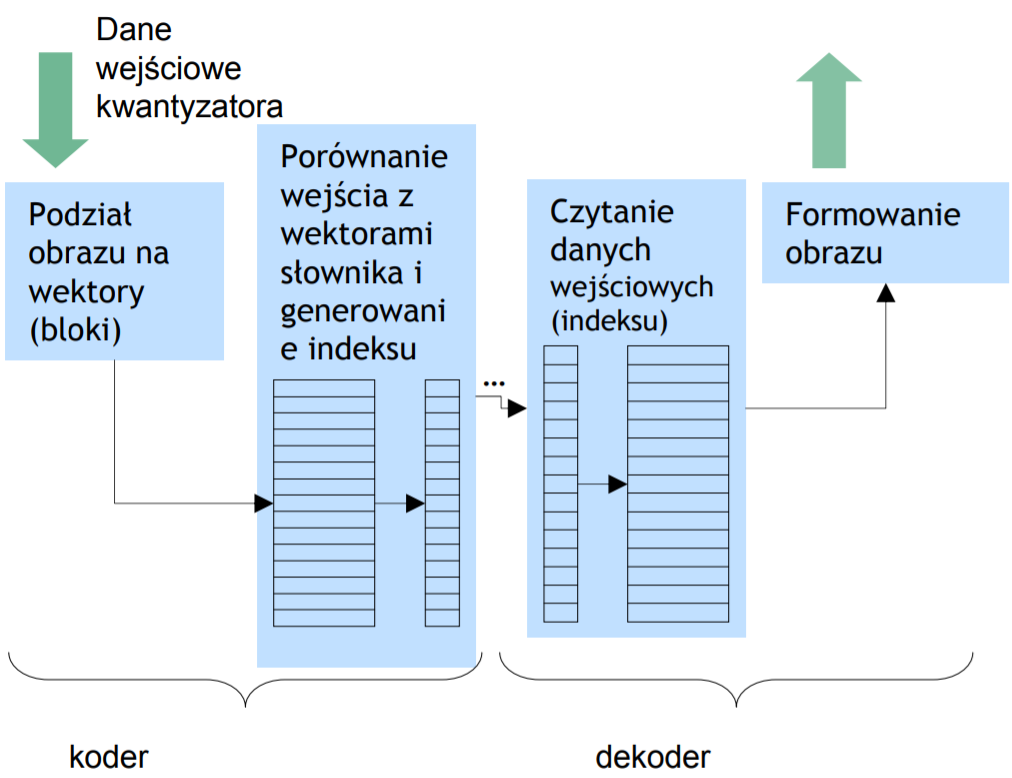
\includegraphics[width=0.6\textwidth]{images/schemat_kwantyzatora.png}
    \caption{Ogólny schemat pracy kwantyzatora. Źródło \cite{mwilczewski}.}
    \label{fig:schemat_kwantyzatora}
\end{figure}

\begin{figure}[H]
    \centering
    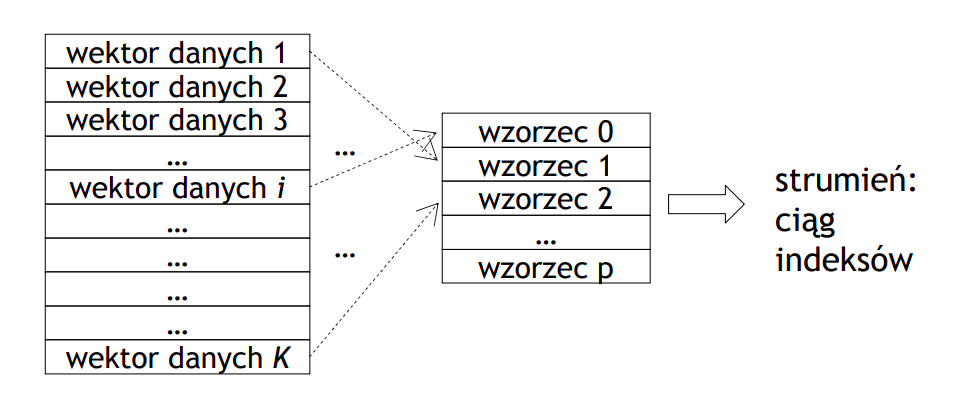
\includegraphics[width=0.6\textwidth]{images/wektory_danych.png}
    \caption{Porównywanie wektorów danych z wektorami ze słownika. Źródło \cite{mwilczewski}.}
    \label{fig:wektory_danych}
\end{figure}

Problemy jakie możemy napotkać podczas kwantyzacji wektorowej:
\begin{enumerate}
  \item Wybór odpowiedniej funkcji odległości w przestrzeni wektorowej.  
  \item Struktura książki kodowej (prosta struktura w postaci tablicy jest nieefektywna do przeglądania).
\end{enumerate}

\subsection{Inicjalizacja książki kodowej}

W procesie kwantyzacji wektorowej ważną rolę odgrywa proces inicjalizacji książki kodowej.
Ma to znaczenie w procesie budowy książki kodowej, gdzie efektywność zależy od początkowych wartości.
Źle dobrane wartości inicjalizacyjne mogą przeszkadzać w zbieżności algorytmu.

Podstawowymi metodami inicjalizacji książki kodowej są:

\begin{enumerate}
  \item metoda losowania,
  \item metoda grupowania najbliższych sąsiadów (ang. PNN - pairwise nearest neighbour),
  \item metoda rozdzielania (ang. splitting).
\end{enumerate}

Metoda losowa polega na wylosowaniu $N$ wektorów, gdzie $N$ jest liczba całkowitą. 
Rozwiązanie jest wykorzystywane gdy posiada się mało informacji na temat danych wektorowych lub liczy się
szybkość inicjalizaci. 

Druga metoda tworzenie słownika, czyli metoda grupowania najbliższych sąsiadów pozwala osiągnąć lepsze wyniki niż metoda losowa, 
ale za to jest dużo bardziej czasochłonna. 
Polega ona na tworzeniu coraz liczniejszych grup zaczynając od jednoelementowej, związanej z każdym wektorem sekwencji. 
W następnych iteracjach wyznaczamy najbliższe grupy, czyli liczymy odległości pomiędzy środkami poszczególnych grup. 
Następnie dwie najbliższe sobie grupy zostają połączone tak aby zmniejszać liczbę grup.

Algorytm metody PNN:

\todo{Poprawić opis metody PNN}

\begin{enumerate}
 \item Rozważamy zestaw $N$ wektorów treningowych w przestrzeni euklidesowej $K$-wymiarowej. 
   Zadaniem konstrukcji książki kodowej jest odnalezienie zestawu wektorów kodowych $M$ poprzez minimalizację 
   średniej kwadratowej odległości $M$ pomiędzy wektorami treningowymi $T_{i}$ a ich reprezentatywnymi wektorami z książki kodowej $C_{j}$:

\begin{equation}
D = \frac{1}{N} \sum_{j=1}^M \sum_{T_{i}\in\mathbb{S_{j}}} ||T_{i} - C_{j}||^2
\end{equation}

\item $S=S_{1}$,...,$S_{m}$ definiuje grupowanie zestawu treningowego $T$. 
  Dla danego kodeksu $C$. 
  Optymalne grupowanie może być zbudowane poprzez przypisanie każdego wektora $T_{i}$ do klastra $j_{0}$ dla którego:

\begin{equation}
||T_{i} - C_{j0}||^2 = \displaystyle \min_{j_1,\dots ,M} ||T_{i} - C_{j}||^2
\end{equation}

\item Metoda ta rozpoczyna się od zainicjowania każdego wektor szkoleniowy $T_{i}$ jako własny klaster $S_{i}$. 
  Na każdym etapie algorytmu, dwa najbliższe klastry ($S_{a}$ i $S_{b}$) są przeszukiwane i łączone. 
  Odległość (koszt połączenia) $d$ pomiędzy dwoma klastrami jest definiowany jako wzrost zniekształcenia książki kodowej w przypadku połączenia klastrów:

\begin{equation}
d(S_{a}, S_{b}) = \frac{n_{a}n_{b}}{n_{a} + n_{b}} || C_{a} - C_{b} ||^2
\end{equation}

\item Wybrane klastry $S_{a}$ i $S_{b}$ są następnie łączone. Wielkość połączonego klastra $S_{a}$ + $S_{b}$ wynosi $n_{a+b} = n_{a} + n_{b}$, 
  a odpowiednim wektorem kodu jest centroid wektorów szkoleniowych w klaster. Można go obliczyć jako średnią ważoną $C_{a}$ i $C_{b}$:

\begin{equation}
C_{a + b} = \frac{n_{a}C_{a} + n_{b}C_{b}}{n_{a} + n_{b}}
\end{equation}

\item Wystarczy zatem utrzymać tylko centroidy klastra $C_{i}$ i rozmiary klastrów $n_{i}$ w realizacji algorytmu. 
  Proces łączenia jest powtarzany do momentu aż książka kodowa osiągnie rozmiar $M$. 

\end{enumerate}

gdzie:
\begin{itemize}[label=]
    \item $T$ - Zestaw $N$ wektorów treningowych $T = {[T_{1}, T_{2}, \dots, T_{N}]}$
    \item $C$ - Książka kodowa wektorów $C = {[C_{1}, C_{2}, \dots, C_{m}]}$
    \item $M$ - Rozmiar książki kodowej
    \item $K$ - Wymiar wektorów
    \item $S_{i}$ - Klaster (zestaw) wektorów treningowych $n_{i}$
    \item $NN_{i}$ - Indeksy najbliższego sąsiada klastra $S_{i}$
    \item $d_{i}$ - Zwiększenie zniekształcenia w przypadku połączenia klastrów $S_{i}$ i $NN_{i}$
    \item $R_{i}$ - Wskaźnik ważności. $R_{i}$ = true jeśli $d_{i}$ jest poprawne.
    \cite{tkaukoranta} 
\end{itemize}

Ostatnia wymieniona metoda jaką jest metoda rozdzielania polega na szukaniu optymalnej książki.
Konstrukcja rozpoczyna się od pojedynczego wektora – centroidu zbioru uczącego.
W $i$-tym kroku dokonywany jest (w drodze dodawania zaburzenia) podział każdego z wektorów kodowych na dwa wektory.
Po takim rozdzieleniu uzyskana konfiguracja regionów decyzyjnych jest optymalizowana przez algorytm LBG, po czym dokonywany jest kolejny rozdział, etc.

\begin{figure}[H]
    \centering
    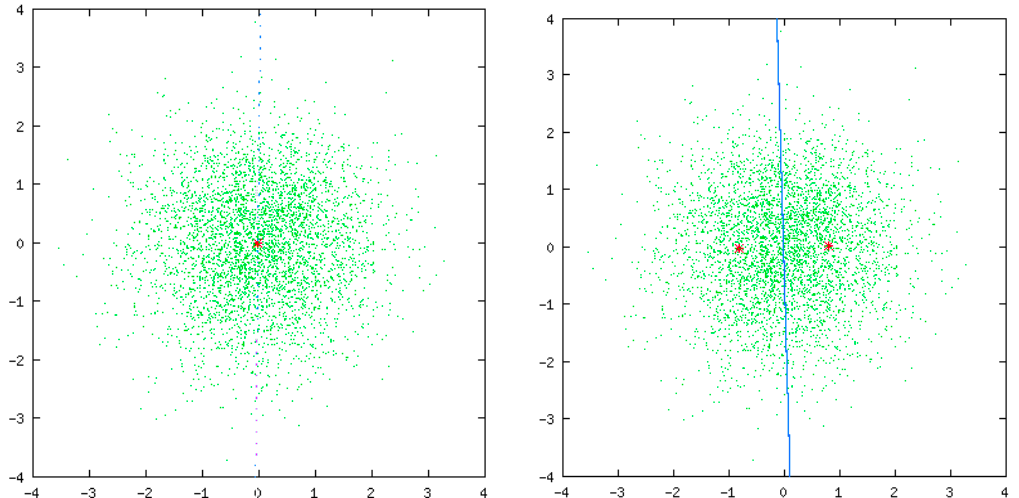
\includegraphics[width=0.6\textwidth]{images/rodzielania_1.png}
    \caption{Konstrukcja słownika metodą rozdzielania. Kolejne etapy konstrukcji wektorów kodowych 
    (zaznaczone czerwonymi punktami) na zbiorze uczącym (zaznaczony kolorem zielonym). Źródło \cite{mwilczewski}.}
    \label{fig:rozdzielania_1}
\end{figure}

\begin{figure}[H]
    \centering
    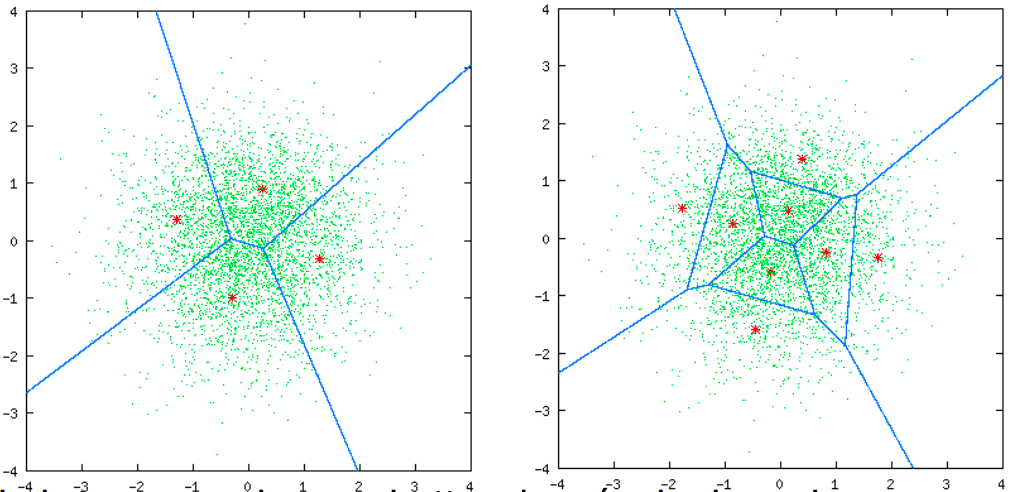
\includegraphics[width=0.6\textwidth]{images/rodzielania_2.png}
    \caption{Konstrukcja słownika metodą rozdzielania. Kolejne etapy konstrukcji wektorów kodowych 
    (zaznaczone czerwonymi punktami) na zbiorze uczącym (zaznaczony kolorem zielonym). Źródło \cite{mwilczewski}.}
    \label{fig:rozdzielania_2}
\end{figure}

\subsection{Algorytmy inicjalizowania słownika}

\subsubsection{Algorytm popularności}

Algorytm popularności jest prostym algorytmem generacji książki kodowej, który charakteryzuje się:

\begin{itemize}
  \item wektorami kodowymi staje się ustalona liczba wektorów danych najczęściej występujących 
    w obrazie (konieczne jest ustalenie progu liczby wystąpień),
  \item algorytm wyróżnia się stosunkowo małą złożonością obliczeniową i prostotą implementacji,
  \item wadą podstawowej wersji algorytmu popularności jest wprowadzanie do książki kodowej podobnych wartości (dominujących). 
    Redukcję rozmiaru książki uzyskać można przez usunięcie bliskich (w sensie przyjętej metryki) wektorów i 
    wprowadzenie kolejnych wektorów pod względem liczby wystąpień.

\begin{figure}[H]
    \centering
    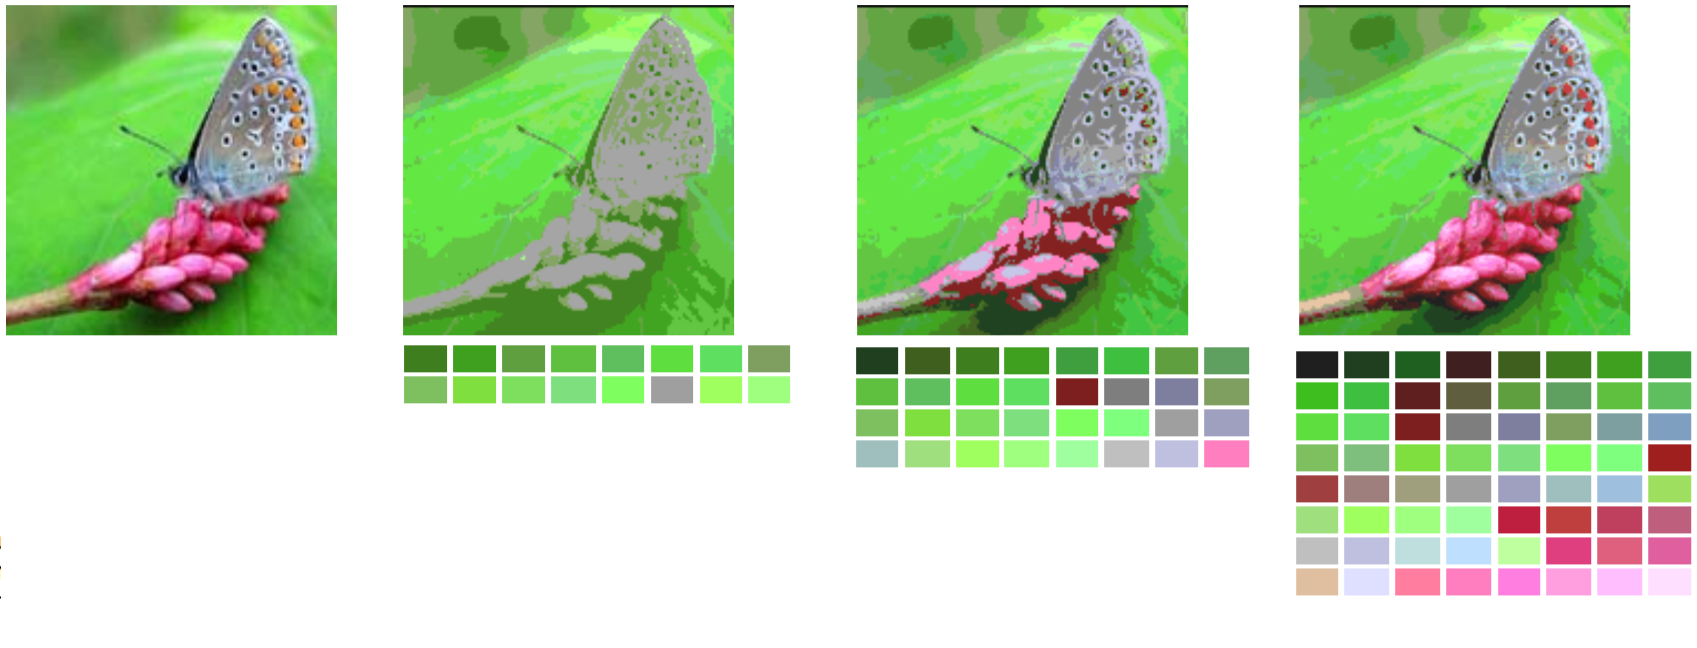
\includegraphics[width=0.6\textwidth]{images/motyle_2.png}
    \caption{Przykład kwantyzacji wektorowej przeprowadzonej z książką kodową skonstruowaną zgodnie z algorytmem popularności.
      Efekt kwantyzacji wektorowej z książkami kodowymi rozmiaru odpowiednio: 16, 32 oraz 64. Źródło \cite{aprzelaskowski}.}
    \label{fig:motyle_2}
\end{figure}
 
\end{itemize}

\subsubsection{Wektorowa kwantyzacja blokowa (BTC)}

Wektorowa kwantyzacja blokowa (BTC) charakteryzuje się:

\begin{itemize} 
\item W przypadku podstawowej wersji metody BTC każdy skwantyzowany blok obrazu reprezentowany jest jako strumień 
  bitowy przez mapę bitową zawierającą $n^{2}$ bitów oraz dwa bajty reprezentujące poziomy rekonstrukcji. W takim przypadku:
     \begin{itemize}
        \item liczba wszystkich możliwych map bitowych jest równa $n^{2}$ = 65536,
        \item nie wszystkie z nich występują w każdym obrazie cyfrowym, np. ze względu na rozmiar obrazu oraz korelacje danych obrazowych, 
     \end{itemize}
\item jednym z możliwych sposobów wykorzystania powyższych obserwacji do kompresji obrazu jest 
  kwantyzacja wektorowa map bitowych, tzn. reprezentacja zbioru wszystkich możliwych map bitowych przez niewielki jego podzbiór (słownik),
\item w fazie indeksowania, każda z map bitowych stworzonych dla kolejnych bloków obrazu porównywana jest ze zbiorem map w słowniku. 
  Prostą miarą podobieństwa map jest liczba miejsc na których porównywane mapy różnią się. 
  Mapą najbardziej podobną do zadanej jest mapą minimalizującą tak zdefiniowaną miarę,
\item wykorzystanie zbioru map stanowiących słownik zwiększa stopień kompresji. 
  Przykład: w przypadku bloków 4x4 oraz 32 elementowego słownika 16 bitów reprezentujących 
  elementy oryginalnej mapy można zastąpić 5 bitowym indeksem słownika. Zwiększa to stopień kompresji z CR=4.0 do CR=6.09.
\end{itemize}

\subsection{Algorytmy budowy słownika}

\subsubsection{Algorytm Lindego-Buza-Graya}

Algorytm Lindego-Buza-Graya (LBG), powstał 1980, służy on do generowania książki kodowej. Przebieg algorytmu przedstawia się następująco:

\begin{itemize} 
\item określić wektory danych zbioru uczącego. Spośród wszystkich $N$ wektorów wejściowych 
  wybierz losowo $K$ wektorów stanowiących wstępną wersję słownika,
\item korzystając z metryki euklidesowej, $d(X,Y)$, dokonaj klasteryzacji wektorów danych wokół słów kodowych bieżącej wersji słownika
     \begin{itemize}
        \item bierzemy każdy kwadrat z obrazu o rozmiarze $(4x4)$ i sprawdzamy, któremu reprezentantowi ze słownika jest najbliżej do 
        naszego kwadratu. Każdy piksel wewnątrz tego kwadratu porównujemy ze sobą i liczymy ich różnice w kwadracie.
        
		\begin{equation}
		d(B_{m}, C_{i}) < d(B_{m}, C_{j})
		\end{equation}
		
		gdzie:
		\begin{itemize}[label=]
    		\item $B_{m}$ - blok obrazu,
    		\item $C_{i}$ - słowo kodowe ze słownika
    		\item $C_{j}$ - kolejne słowo kodowe ze słownika
		\end{itemize}	        
        
        \item następnie sumujemy różnicę 16 kwadratów
        \item sprawdzamy kwadrat obrazu z każdym reprezentantem słownika centroid
        \item przypisujemy wybrany kwadrat do reprezentanta słownika
     \end{itemize}
\item wyznaczamy globalny błąd kwantyzacji popełniony w bieżącej iteracji czyli wykonujemy sumowanie wszystkich 
  znalezionych odległości miedzy poszczególnymi kwadratami a centroidami 
 
\begin{equation}
e = \sum_{i=1}^K \sum_{x\in\mathbb{R}} d(X, Y_{i}) 
\end{equation}

\item sprawdzić czy popełniany błąd zmienił się względem poprzedniej iteracji jeśli nie ma to kończymy algorytm 
  (dla uproszczenia ustaliliśmy, że liczbę iteracji będzie podawana z ręki)
\item wyznacz centroidy każdego regionu decyzyjnego i uczyń je wektorami kodowymi kolejnej iteracji słownika. Przejdź do kroku 2. 
\end{itemize}
 
Problemy tego algorytmu:

\begin{itemize}
	\item wrażliwość na inicjalną postać książki kodowej 
	\item problem pustych przedziałów 
\end{itemize}

\paragraph{Sparametryzowany wzór pliku wynikowego}
Plik wynikowy kwantyzacji wektorowej składa się ze słownika o określonej długości $K$ oraz wartości przyporządkowanych indeksów do każdego bloku. Każdy element słownika reprezentowany jest przez wektor o długości $v$, który zapisywany jest na $v \cdot 8$ bitach.

Każdy blok jest opisywany przez indeks, który można zapisać na $log_2(K)$ bitach. Przykładowo dla słownika o $512$ elementowego każdy wektor będzie reprezentowany przez indeks zapisany na $9$ bitach.


Dla rozmiaru o wielkości $m \times n$, długości słownika $K$ i wielkości wektora wyrażanej przez $v$ otrzymujemy słownik o rozmiarze

\begin{equation}
	\textrm{dict\_size} = K \cdot v \cdot 8 \quad \textrm{[bitów]}.
\end{equation}

Każdy blok przechowujący indeks ma rozmiar:

\begin{equation}
	\textrm{block\_size} = log_2(K)  \quad  \textrm{[bitów]}.
\end{equation}

Dla obrazie o wielkości $m \times n$ otrzymujemy $\frac{mn}{v}$ bloków. Cały obraz zapisany na: 

\begin{equation}
	\textrm{file\_size} = \textrm{dict\_size} + \frac{mn}{v} \cdot \textrm{block\_size}  \quad  \textrm{[bitów]}.
\end{equation}

\subsubsection{Kwantyzacja wektorowa z usuniętą średnią}

Kwantyzacja wektorowa z usuniętą średnią (MRVQ) jest zmodyfikowaną wersją schematu VQ. 
Celem MRVQ jest zapewnienie lepszej jakości obrazu niż VQ. 
Aby osiągnąć ten cel, do kodowania każdego bloku obrazu w MRVQ wykorzystuje się wartość średnią bloku oraz indeks wektora resztkowego. 
Schemat MRVQ składa się z trzech procedur: generowania książki kodów resztkowych, kodowania obrazu i dekodowania obrazu.
Aby wygenerować resztkową książkę kodową RCB z N resztkowych słów kodowych dla MRVQ, zastosowano algorytm LBG. 
Zamiast obrazów szkoleniowych używanych do projektowania książki kodowej VQ, do projektowania książki kodowej MRVQ wykorzystuje się wektory resztkowe. 
Po pierwsze, bloki obrazów treningowych są generowane przez podzielenie obrazów treningowych na nienakładające się 
na siebie bloki obrazów o $4 \times 4$ pikseli. 
Każdy blok obrazów treningowych składający się z $4 \times 4$ pikseli może być postrzegany jako wektor $k$-wymiarowy, gdzie $k=4 \times 4$. 
Każdy wektor treningu jest przekształcany na jeden wektor reprezentowany poprzez odjęcie jego średniej wartości bloku od wartości każdego piksela. 
Następnie algorytm LBG opisany w sekcji 2.5.1 jest wykorzystywany do projektowania książki 
kodów resztkowych RCB = ( $rcw_{0}$, $rcw_{1}$, \dots , , $rcw_{N-1}$ ) przy użyciu wektorów resztkowych.

Wartość średnia bloku $bm$ dla każdego bloku obrazu $x$ jest obliczana za pomocą wyrażenia: 

\begin{equation}
bm = \frac{1}{k} \sum_{i=0}^{k-1} x_{i}
\end{equation}

Następnie generowany jest pozostały wektor $rv$ poprzez odjęcie wartości $bm$ od każdej wartości piksela w $x$.
Przeszukiwane jest najbliższe pozostałe słowo kodowe w $RCB$ dla pozostałego wektora $rv$ i zapisywany jest indeks
najbliższego pozostałego słowa kodowego \cite{meanremovedVQ}. 

\todo{Sparametryzowany wzór na długość pliku wynikowego}

\subsection{Wykorzystywane metryki}

\subsubsection{PSNR}

Szczytowy stosunek sygnału do szumu, (ang. \emph{peak signal-to-noise ratio (PSNR)}) – stosunek maksymalnej mocy sygnału do mocy szumu zakłócającego ten sygnał.  

Najczęściej PSNR stosowany jest do oceny jakości kodeków wykorzystujących stratną kompresję obrazków. 
W takim przypadku sygnałem są nieskompresowane dane źródłowe, a szumem – artefakty (zniekształcenia) spowodowane zastosowaniem kompresji stratnej. 

W celu wyznaczenie PSNR, należy najpierw obliczyć współczynnik MSE (błąd średniokwadratowy) bazując na obu porównywanych obrazkach za pomocą wzoru:

\begin{equation}
MSE = \frac{1}{N \cdot M} \sum_{i=1}^N \sum_{j=1}^M ([f(i, j) - f^{'}(i, j)]^2
\end{equation}

gdzie:
\begin{itemize}[label=]
    \item $N, M$ - wymiary obrazu w pikselach,
    \item $f(i, j)$ - wartość piksela o współrzędnych $i(i, j)$ obrazu oryginalnego
    \item $f^{'}(i, j)$ - wartość piksela o współrzędnych $i(i, j)$ obrazu skompresowanego
\end{itemize}

Następnie wyliczoną wartość MSE należy podstawić do końcowego wzoru: 

\begin{equation}
PSNR = 10 \cdot \log_10 \frac{[max(f(i,j))]^2}{MSE}
\end{equation}

gdzie:
\begin{itemize}[label=]
    \item $max(f(i,j))$ - wartość maksymalna danego sygnału; w przypadku obrazów zwykle jest to wartość stała,
      np. dla obrazów monochromatycznych o reprezentacji 8-bitowej wynosi 255.
\end{itemize}

\subsubsection{SSIM}

Podobieństwo strukturalne miarą indeksu (ang. \emph{structural similarity index measure}) jest to metoda, która służy 
do pomiaru podobieństwa między dwoma obrazami. Indeks $SSIM$ to pomiar jakości obrazu bazowego (nieskompresowanego) 
do obrazu po przekształceniach. SSIM to model oparty na percepcji, który traktuje degradację obrazu jako postrzeganą zmianę
w informacjach strukturalnych, przy jednoczesnym uwzględnieniu ważnych zjawisk percepcyjnych, w tym zarówno terminów maskowania 
luminancji, jak i maskowania kontrastu. Różnica w stosunku do innych technik, takich jak $MSE$ lub $PSNR$,
polega na tym, że te podejścia szacują błędy bezwzględne. Idea informacji strukturalnych polega na tym, że piksele mają silne współzależności,
zwłaszcza gdy są znajdują się blisko siebie w przestrzenni. Zależności te niosą ważne informacje o strukturze obiektów \mbox{na scenie wizualnej \cite{channappayya2008rate}.}

Algorytm SSIM:

\begin{equation}
SSIM(x, y) = \frac{(2\mu_{x}\mu_{y} + c_{1}) (2\delta_{xy} + c_2)}{(\mu_{x}^2 + \mu_{y}^2 + c_{1}) (\delta_{x}^2 + \delta_{x}^2 + c_2)}
\end{equation}

gdzie:
\begin{itemize}[label=]
    \item $\mu_{x}$ - średnia x
    \item $\mu_{y}$ - średnia y
    \item $\delta_{x}^2$ - odchylenie od x
    \item $\delta_{y}^2$ - odchylenie od y
    \item $\delta_{xy}$ - kowariancja x i y
\end{itemize}

\subsubsection{FSIM}

Zastosowanie wskaźnika podobieństwa funkcji (ang. \emph{A Feature Similarity Index}) do oceny jakości obrazu, 
jest zagadnieniem skoncentrowanym wokół pomiaru podobieństwa między dwoma obrazami.
W celu interpretacji danego wskaźnika wymagane jest wyjaśnienie dwóch pojęć: zgodności fazowej (PC) oraz wielkości gradientu (GM) \cite{fsim_theory}.

\paragraph{Zgodność fazowa (ang. \emph{Phase Congruency}) (PC):}
Nową metodą wykrywania cech obrazu jest zgodność fazowa. Ważną cechą charakterystyczną zgodności fazowej jest to,
że jest stała dla zmiennych wartości światła na obrazie. Wskaźnik ten podkreśla cechy obrazu w częstotliwości fazowej. 
Jest to wartość niezmienna dla kontrastu. Na podstawie metody opisanej przez P. Kovesi, szeroko stosowanej w literaturze, 
można wyznaczyć wzór na obliczanie mapy zgodności fazowej dla obrazu \cite{pc}:

\begin{equation}
PC(x) = E(x) / (\varepsilon + \sum\limits{_{n}} A_n(x))
\end{equation}

\paragraph{Wielkość gradientu  (ang. \emph{Gradient Magnitude}) (GM):}
Obliczanie gradientu obrazu jest bardzo tradycyjnym tematem w cyfrowym przetwarzaniu obrazu. 
Maski splotu są używane do wyrażania operatorów gradientu. Istnieje wiele masek konwolucyjnych do pomiaru gradientów. 
Jeśli $f(x)$ jest obrazem, a $Gx$ oraz $Gy$ to odpowiednio jego gradient poziomy i pionowy. 
Wtedy wielkośc gradientu $f(x)$ można zdefiniować następująco \cite{gm}:

\begin{equation}
\sqrt{G^2_x+G^2_y}
\end{equation}

\paragraph{Algorytm FSIM \cite{fsim_alg}:}
Obliczanie indeksu FSIM składa się z dwóch etapów. 
W pierwszym etapie obliczana jest lokalna mapa wartości, a następnie w drugim etapie łączy się lokalne mapy podobieństwa w jeden wynik.
Wyliczany jest następnie oddzielny pomiar podobieństwa cech pomiędzy $f_1(x)$ i $f_2(x)$ obliczając wartości po dwie 
składowe na pomiar dla PC lub GM. Najpierw, miara podobieństwa dla $PC_1 (x)$ i $PC_2(x)$ jest zdefiniowana jako:

\begin{equation}
S_{PC}(x) = \frac{2PC_1(x) \cdot PC_2(x) + T_1}{PC^2_1(x) + PC^2_2(x) + T_1}
\end{equation}

gdzie:
\begin{itemize}[label=]
    \item $T_1$ - dodatnia stała zwiększająca stabilność $S_PC$
\end{itemize}

Podobnie porównuje się wartości GM $G_1(x)$ i $G_2(x)$, a miarę podobieństwa definiuje się jako:

\begin{equation}
S_G(x) = \frac{2G_1(x) \cdot G_2(x) + T_2}{G^2_1(x) + G^2_2(x) + T_2}
\end{equation}

gdzie:
\begin{itemize}[label=]
    \item $T_2$ - dodatnia stała zależna od dynamicznego zakresu wartości $GM$
\end{itemize}

Następnie $S_{PC}(x)$ i $S_G(x)$ są łączone, aby uzyskać podobieństwo $S_L(x)$ z $f_1(x)$ i $f_2(x)$. $S_L(x)$ jest definiowane jako:

\begin{equation}
S_L(x) = [S_{PC}(x)]^\alpha \cdot [S_G(x)]^\beta
\end{equation}

gdzie:
\begin{itemize}[label=]
    \item $\alpha$, $\beta$ - parametry używane do dostosowania względnego znaczenia cech PC i GM
\end{itemize}

Po uzyskaniu podobieństwa $S_L(x)$ w każdym miejscu $x$ można obliczyć całkowite podobieństwo między $f_1$ i $f_2$. 
Jednak różne lokalizacje mają różny wpływ na postrzeganie obrazu przez HVS (ludzki system widzenia). 
Na przykład lokalizacje krawędzi przekazują ważniejsze informacje wizualne niż lokalizacje na gładkim obszarze. 
Ponieważ ludzka kora wzrokowa jest wrażliwa na struktury zgodne fazowo \cite{kora_wzrokowa}, wartość PC w danej 
lokalizacji może odzwierciedlać prawdopodobieństwo, że jest to dostrzegalnie istotny punkt obrazu. 
Intuicyjnie, dla danej lokalizacji $x$, jeśli którykolwiek wartość z $f_1(x)$ i $f_2(x)$ ma znaczącą wartość PC, 
oznacza to, że ta pozycja $x$ będzie miała duży wpływ na HVS w ocenie podobieństwa między $f_1$ i $f_2$. 
Dlatego używa się wartości maksymalnych $PC_m(x) = max (PC_1(x), PC_2(x))$, aby nadać wagę parametrowi $S_L(x)$ w 
ogólnym podobieństwie między $f_1$ i $f_2$, i odpowiednio zdefiniowano indeks FSIM między $f_1$ i $f_2$ w sposób przedstawiony poniżej:

\begin{equation}
{FSIM} = {{\sum\limits {_{{\bf x} \in \Omega } {S_{L}}({\bf x}) \cdot PC_{m}({\bf x})} } \over {\sum\limits {_{{\bf x} \in \Omega } PC_{m}({\bf x})}}}
\end{equation}

gdzie:
\begin{itemize}[label=]
    \item $\Omega$ - dziedzina przestrzeni obrazu
\end{itemize}

\subsubsection{CR}

\subsubsection{RMSE}

Podstawowy błąd średniokwadratowy (RMSE) - jest to reguła, która mierzy średnią wielkość błędu. Jest to pierwiastek kwadratowy każdej różnicy między prognozowaną a odpowiadającą jej wartościom, podniesiona do kwadratu, a następnie uśredniona w próbie. Ponieważ błędy są podnoszone do kwadratu, zanim zostaną uśrednione, sprawia to, że RMSE nadaje stosunkowo dużą wagę dużym błędom. Oznacza to, że RMSE jest najbardziej przydatny, gdy duże błędy są szczególnie niepożądane.

Wzór RMSE:

\begin{equation}
RMSE = \sqrt{\frac{1}{n} \sum_{j=1}{n} (y_{j} - \hat{y_{j}} )^2}
\end{equation}

gdzie:
\begin{itemize}[label=]
    \item $n$ - średnia próby,
    \item $y_{j}$ - prognozowana wartość błędu,
    \item $\hat{y_{j}}$ - rzeczywista wartość błędu \cite{rmse}.
\end{itemize}

\section{Badania}

\subsection{Algorytm LBG z losową inicjalizacją słownika}

Przeprowadzono badania na wszystkich dostarczonych obrazach badawczych. Kwantyzację przeprowadzono na blokach o rozmiarach $4 \times 4$ oraz dla książki
kodowej o długości $512$ elementów. Dane zebrano w \mbox{tablicy \ref{tab:lbg_random}} i podsumowano w tablicy \mbox{\ref{tab:lbg_summary}}.

% Please add the following required packages to your document preamble:
% \usepackage{booktabs}
\begin{table}[ht]
\centering
\begin{tabular}{@{}lrrrr@{}}
\toprule
Obraz              & PSNR {[}dB{]} & SSIM   & MSE      & NRMSE  \\ \midrule
Aerial.bmp         & 31.6636       & 0.8747 & 137.5262 & 0.0634 \\
airfield.bmp       & 30.8671       & 0.7938 & 156.1186 & 0.0804 \\
airplane.bmp       & 34.6427       & 0.9236 & 49.7802  & 0.0382 \\
baboonTMW.bmp      & 29.9951       & 0.7893 & 219.1716 & 0.1089 \\
balloon.bmp        & 39.3125       & 0.9533 & 10.6350  & 0.0292 \\
balloon\_noise.bmp & 39.1234       & 0.9496 & 11.2513  & 0.0302 \\
BARB.bmp           & 32.2852       & 0.8837 & 89.9736  & 0.0790 \\
BARB2.bmp          & 32.1664       & 0.8853 & 89.5440  & 0.0754 \\
barb512.bmp        & 32.1491       & 0.8806 & 95.2525  & 0.0754 \\
BOARD.bmp          & 36.4226       & 0.9313 & 28.9137  & 0.0459 \\
boat512.bmp        & 32.8108       & 0.8650 & 71.7116  & 0.0614 \\
boats.bmp          & 34.3485       & 0.9128 & 43.6047  & 0.0509 \\
bridge.bmp         & 30.3832       & 0.8038 & 157.6636 & 0.0994 \\
bridge256.bmp      & 30.3125       & 0.8323 & 141.0575 & 0.0946 \\
camera256.bmp      & 33.7937       & 0.9055 & 94.8728  & 0.0726 \\
couple.bmp         & 32.4539       & 0.8631 & 74.4537  & 0.0670 \\
couple256.bmp      & 35.5769       & 0.9339 & 29.8176  & 0.1196 \\
crowd512.bmp       & 33.4139       & 0.9171 & 64.5795  & 0.0815 \\
EARTH.bmp          & 33.5174       & 0.9325 & 65.9923  & 0.0842 \\
elaine.bmp         & 33.1995       & 0.8364 & 40.8950  & 0.0444 \\
ELIF.bmp           & 37.8132       & 0.9587 & 16.7079  & 0.0544 \\
finger.bmp         & 29.9399       & 0.9008 & 131.6425 & 0.0925 \\
FROG512.BMP        & 29.8664       & 0.7281 & 168.3580 & 0.1013 \\
GIRL.bmp           & 35.2442       & 0.9169 & 26.8099  & 0.0367 \\
GOLD.bmp           & 33.3489       & 0.8668 & 45.4286  & 0.0589 \\
GOLDHILL.BMP       & 32.9129       & 0.8629 & 52.1809  & 0.0590 \\
harbour512.bmp     & 32.2399       & 0.8563 & 127.0800 & 0.0854 \\
HOTEL.bmp          & 33.3766       & 0.8960 & 67.1312  & 0.0753 \\
lax512.bmp         & 30.9269       & 0.7800 & 160.8272 & 0.1421 \\
lenaTMW.bmp        & 33.6248       & 0.8704 & 52.2250  & 0.0644 \\
lennagrey.bmp      & 34.6031       & 0.8994 & 39.0316  & 0.0471 \\
man512.bmp         & 33.0232       & 0.8705 & 64.1381  & 0.0660 \\
noisesquare.bmp    & 32.9291       & 0.8254 & 35.6925  & 0.0311 \\
OMAHA.bmp          & 29.9031       & 0.8378 & 327.2889 & 0.1044 \\
peppersTMW.bmp     & 34.2263       & 0.8743 & 42.6578  & 0.0497 \\
SAILBOAT.bmp       & 32.9982       & 0.8771 & 64.4069  & 0.0592 \\
seismic.bmp        & 39.9778       & 0.9726 & 7.4695   & 0.0213 \\
SENA.bmp           & 37.5456       & 0.9542 & 15.2120  & 0.0435 \\
SENSIN.bmp         & 35.3720       & 0.9468 & 23.9566  & 0.0455 \\
shapes.bmp         & 38.4559       & 0.9612 & 22.2232  & 0.0534 \\
SINAN.bmp          & 36.5850       & 0.9493 & 18.1502  & 0.0325 \\
Tank512.bmp        & 33.6339       & 0.8500 & 37.7513  & 0.0455 \\
Truck512.bmp       & 33.9556       & 0.8830 & 33.5212  & 0.0524 \\
woman1.bmp         & 33.3459       & 0.8616 & 65.1471  & 0.0570 \\
woman2.bmp         & 37.7312       & 0.9416 & 13.1210  & 0.0292 \\
ZELDA.bmp          & 36.5893       & 0.9163 & 18.5568  & 0.0368 \\ \bottomrule
\end{tabular}
\caption{Porównanie jakości kwantyzacji algorytmu budowy słownika LBG z losową inicjalizacją słownika dla bloku $4 \times 4$ oraz długości słownika $512$.}
\label{tab:lbg_random}
\end{table}

% Please add the following required packages to your document preamble:
% \usepackage{booktabs}
\begin{table}[H]
\centering
\begin{tabular}{@{}lrrrr@{}}
\toprule
         & PSNR {[}dB{]} & SSIM  & MSE     & NRMSE \\ \midrule
Minimum  & 29.8664       & 0.7281 & 7.4695   & 0.0213 \\
Maksimum & 39.9778       & 0.9726 & 327.2889 & 0.1421 \\
Średnia  & 33.8828       & 0.8853 & 72.8159  & 0.0641 \\ \bottomrule
\end{tabular}
\caption{Przedstawienie wartości minimalnej, maksymalnej oraz uśrednienie wyników dla poszczególnych metryk.}
\label{tab:lbg_summary}
\end{table}

\subsubsection{Wyznaczenie optymalnej liczby iteracji w algorytmie budowy słownika LBG}

\todo{Opisać jak wyznaczono optymalną liczbę iteracji oraz wnioski}

\begin{figure}[H]
\centering
  \centering
  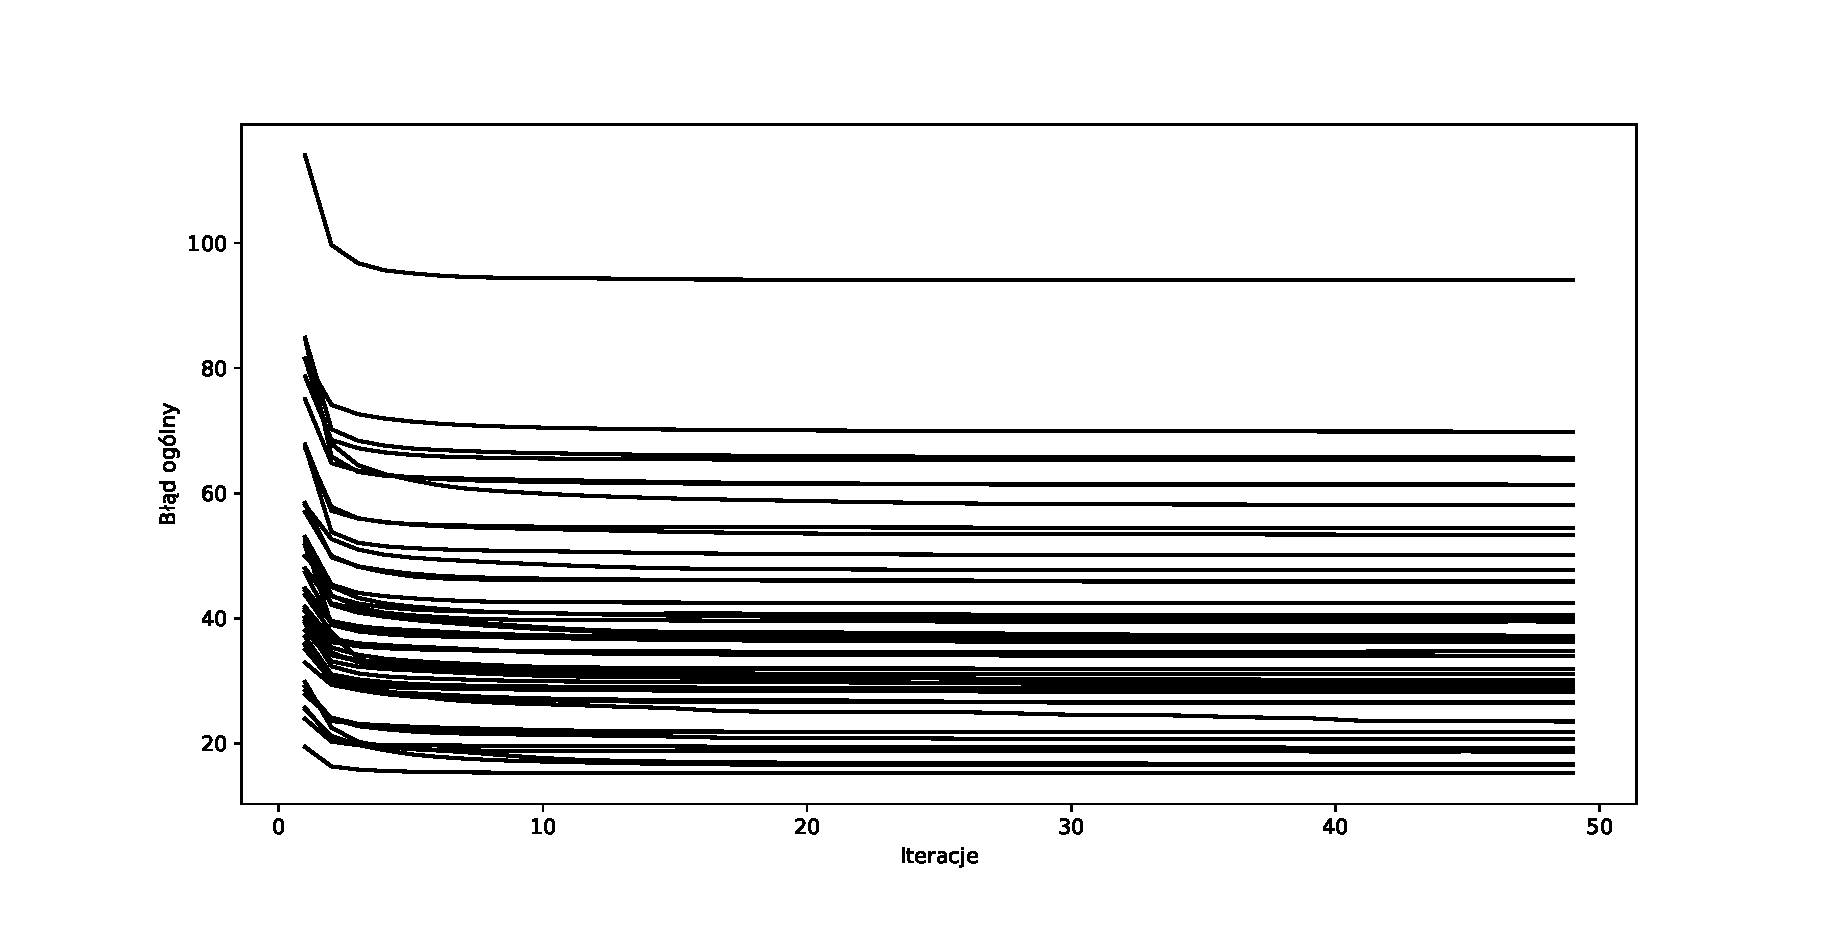
\includegraphics[width=.9\linewidth]{images/lbg_4x4_32_50_iterations.eps}  
  \caption{\todo{Opis wykresu (każda linia to jeden obraz).}}
  \label{fig:lbg_iterations}
\end{figure}

\begin{figure}[H]
  \centering
  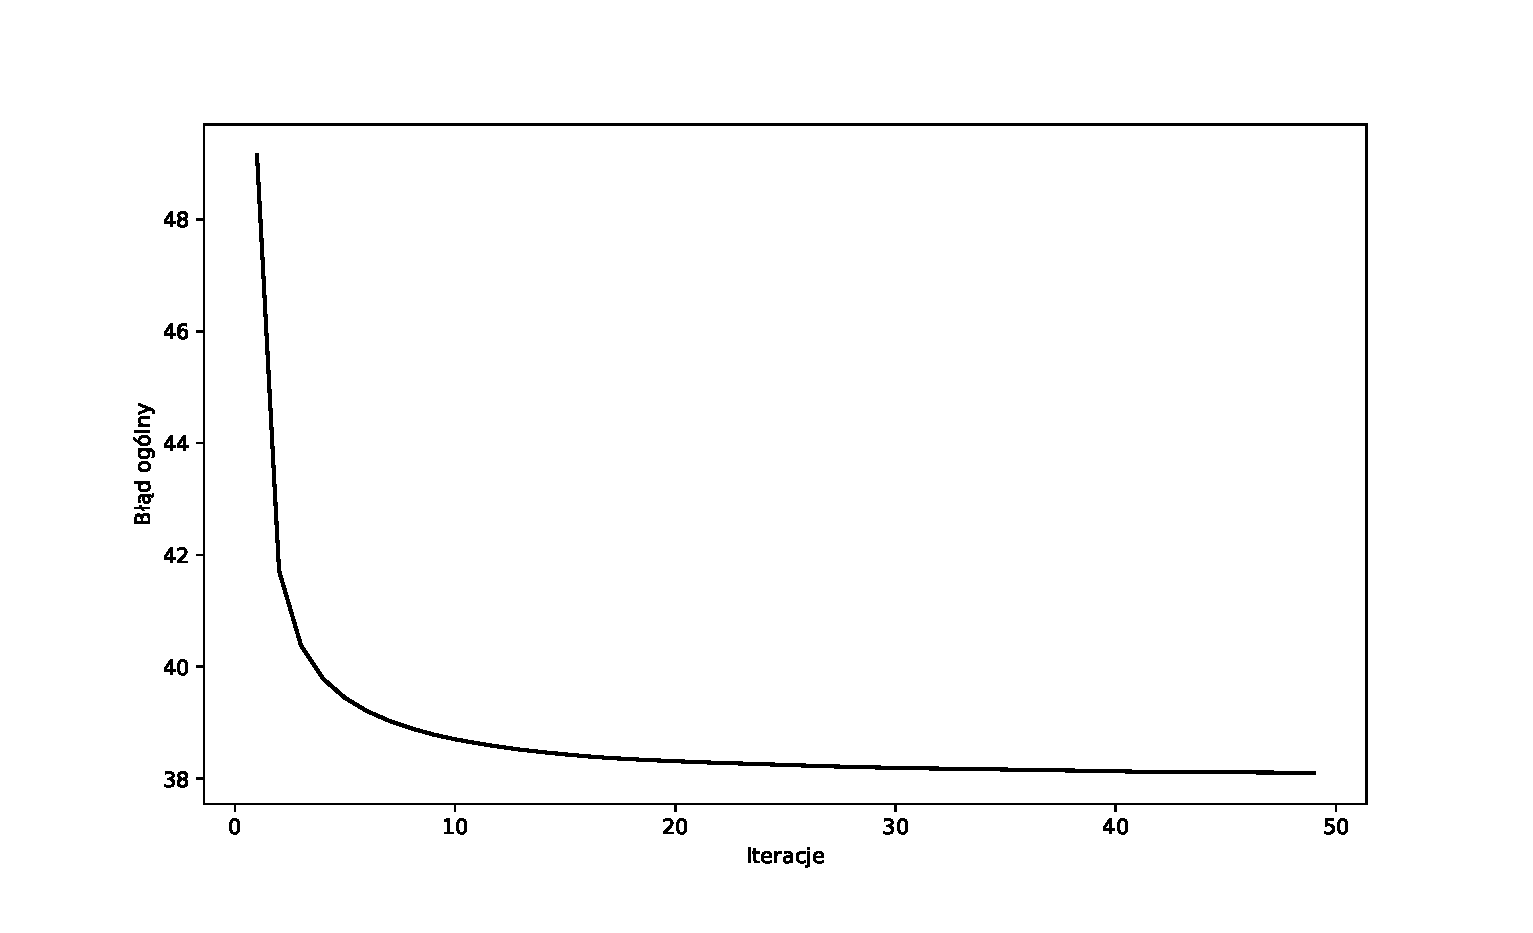
\includegraphics[width=.9\linewidth]{images/lbg_4x4_32_mean_iterations.eps}  
  \caption{\todo{Opis wykresu (średnia z wszystkich obrazów).}}
  \label{fig:lbg_iterations_mean}
\end{figure}


\FloatBarrier
\section{Podsumowanie}

\lipsum[1-3]

\bibliographystyle{unsrt}  
\bibliography{references}  %%% Remove comment to use the external .bib file (using bibtex).
%% and comment out the ``thebibliography'' section.

\end{document}
